\documentclass[conference]{IEEEtran}
\IEEEoverridecommandlockouts

\usepackage[T1]{fontenc}
\usepackage[utf8]{inputenc}
\usepackage{amsmath,amssymb}
\usepackage{booktabs}
\usepackage{multirow}
\usepackage{graphicx}
\usepackage{url}
\usepackage{hyperref}
\usepackage{microtype}
\usepackage{balance}
\usepackage{cite}
\usepackage{algorithm}
\usepackage{algorithmic}
\usepackage{pgfplots}
\pgfplotsset{compat=1.18}

\hypersetup{colorlinks=true,linkcolor=black,citecolor=black,urlcolor=black}

% ──────────────────────────────────────────────────────────────────────────────
\title{Benchmarking Machine Learning for Illicit Bitcoin Detection:\\
Baseline Reproduction, Graph Feature Ablation,\\and Temporal Drift Mitigation on the Elliptic Dataset}

\author{
  \IEEEauthorblockN{Krishika Jain \quad Saanvi [Last Name]}
  \IEEEauthorblockA{Department of [Department Name]\\
    [Institution Name], [City, Country]\\
    \{[email1], [email2]\}@[institution].edu}
}
% ──────────────────────────────────────────────────────────────────────────────

\begin{document}
\maketitle

% ════════════════════════════════════════════════════════════════════════════
\begin{abstract}
Detecting illicit transactions on the Bitcoin blockchain is a critical
challenge for anti-money laundering (AML) compliance and financial
forensics. While existing studies report increasingly high detection
performance using graph neural networks and engineered topological features,
published results remain fragmented across inconsistent evaluation protocols,
non-temporal data splits, and aggregate accuracy metrics that mask
minority-class failures under severe class imbalance.
This paper bridges two complementary strands of work: a structured review
of 23 papers across five methodological paradigms and a rigorous,
seed-replicated empirical evaluation on the full Elliptic benchmark
(203,769 transactions, 49 timesteps, strict temporal split).
Our experiments confirm that a standard Random Forest achieves an
illicit-class $F_1$ of $0.825 \pm 0.001$, faithfully reproducing the
canonical Weber et al.\ benchmark.
A controlled ablation of four graph centrality metrics---in-degree,
out-degree, PageRank, and average neighbour degree---shows a negligible
gain of $+0.002$ in $F_1$, with every graph feature ranking below position
103 out of 169 by Gini importance, challenging widespread claims of
topological feature superiority.
We further expose a catastrophic concept-drift collapse at timestep 43,
consistent with a major darknet-market disruption, where static-model recall
falls to $1.8\%$ and $F_1$ drops to $0.032$.
Evaluating dynamic retraining regimes, we show that an expanding-window
protocol recovers precision to $0.808$ and $F_1$ to $0.164 \pm 0.055$,
whereas a 10-step sliding window starves under label scarcity
($F_1 = 0.087 \pm 0.017$).
Our findings establish practical baselines, expose graph-feature myths,
and provide an operational blueprint for drift-resilient AML pipelines.
\end{abstract}

\begin{IEEEkeywords}
Bitcoin, Anti-Money Laundering, Illicit Transaction Detection, Random Forest,
Graph Neural Networks, Concept Drift, Elliptic Dataset, Temporal Evaluation
\end{IEEEkeywords}

% ════════════════════════════════════════════════════════════════════════════
\section{Introduction}
\label{sec:intro}

Bitcoin and similar public blockchains record every transaction on a
globally readable ledger, yet map each transaction to a pseudonymous
cryptographic address rather than a verified real-world identity.
This pseudonymity has been systematically exploited for ransomware extortion,
darknet marketplace commerce, theft liquidation, and multi-hop money
laundering~\cite{tironsakkul2019probing, harrigan2016unreasonable}.
Regulatory frameworks such as the Financial Action Task Force (FATF)
Travel Rule and the EU's Transfer of Funds Regulation now mandate that
virtual asset service providers implement automated suspicious-transaction
reporting, creating an urgent industrial demand for accurate, temporally
stable machine-learning detectors.

Academic research on illicit cryptocurrency detection has progressed
through three broad waves.
\textit{Heuristic clustering} techniques
\cite{harrigan2016unreasonable, he2022bitcoin, schnoering2024assessing}
group transaction outputs under common ownership using observable
protocol-level patterns, but suffer from false-positive merging in
CoinJoin and payment-batching transactions.
\textit{Taint and flow analysis}
\cite{tironsakkul2019probing, tironsakkul2020tracking, hercog2019taint}
propagates suspicion deterministically through the transaction graph,
yet dilutes rapidly across innocent intermediaries.
\textit{Supervised machine learning and graph neural network (GNN)
approaches}
\cite{weber2019anti, nerurkar2020detecting, guo2023lb,
nicholls2023fraudlens, lin2026wavelet, han2026featuregated}
frame detection as node classification and have recently dominated
published benchmarks.

\subsection{Research Gaps}

Despite this growing body of work, the field suffers from three critical
deficiencies.

\smallskip
\noindent\textbf{(i)~Misleading evaluation metrics.}
Several studies report overall accuracy exceeding 98\%
\cite{asiri2025graph}, masking the fact that the illicit class constitutes
fewer than 3\% of all transactions.
In AML contexts, minority-class precision, recall, and $F_1$-score are
the only operationally meaningful metrics.

\smallskip
\noindent\textbf{(ii)~Unverified graph-feature superiority.}
Numerous studies assert that graph topology is indispensable for high
detection performance, yet few perform controlled ablation experiments
that isolate the marginal contribution of topological features over
strong tabular baselines.

\smallskip
\noindent\textbf{(iii)~Temporal stability is overlooked.}
Existing evaluations commonly use static or random train-test splits,
overlooking sudden behavioural shifts---such as darknet-market
seizures---that cause catastrophic model failures in live deployment.

\subsection{Contributions}

To address these gaps, this paper makes four concrete contributions:
\begin{enumerate}
  \item \textbf{Literature taxonomy.}
    A structured synthesis of 23 core papers across five methodological
    paradigms, contextualized against existing survey works.
  \item \textbf{Rigorous baseline reproduction.}
    Seed-replicated experiments confirming Random Forest at
    $F_1 = 0.825 \pm 0.001$, matching Weber et al.\ \cite{weber2019anti}.
  \item \textbf{Graph-feature ablation.}
    Evidence that four centrality metrics add only $+0.002$ to $F_1$ and
    rank outside the top 100 of 169 features by Gini importance.
  \item \textbf{Drift diagnosis and mitigation.}
    Quantification of the timestep-43 collapse and evaluation of
    expanding-window vs.\ sliding-window retraining, showing expanding
    recovery to $F_1 = 0.164 \pm 0.055$ with precision $0.808$.
\end{enumerate}

The remainder of the paper is structured as follows.
Section~\ref{sec:related} reviews related work.
Section~\ref{sec:dataset} describes the dataset and evaluation protocol.
Section~\ref{sec:method} details the methodology.
Section~\ref{sec:results} presents experimental results.
Section~\ref{sec:discussion} discusses implications, and
Section~\ref{sec:conclusion} concludes.

% ════════════════════════════════════════════════════════════════════════════
\section{Related Work}
\label{sec:related}

We organize related work into five paradigms, using the taxonomy developed
from our structured literature review of 23 papers.

\subsection{Heuristic-Based Address Clustering}

Heuristic-based address clustering is an early approach to analysing Bitcoin
transactions and identifying relationships between addresses.
These methods use observable transaction patterns, such as common-input
ownership and change-address behaviour, to infer whether multiple addresses
may be controlled by the same entity.
Harrigan and Fretter~\cite{harrigan2016unreasonable} examined the
effectiveness of address-clustering heuristics and discussed factors that
can lead to incorrect address merging.
Zhang et al.~\cite{zhang2020heuristic} proposed an improved one-time
change-address heuristic that identifies addresses reused later as
non-change addresses.
He et al.~\cite{he2022bitcoin} combined six heuristic conditions and
proposed an improved change-address detection algorithm to improve
clustering accuracy.
Schnoering et al.~\cite{schnoering2024assessing} examined existing and
newly proposed clustering heuristics and introduced a clustering ratio to
measure the reduction in the number of entities.
Although these methods help identify relationships between Bitcoin addresses,
their results depend on behavioural assumptions and do not establish common
ownership with certainty.

\subsection{Taint Analysis and Transaction Flow}

Taint analysis is used to trace the movement of Bitcoin from known sources,
such as addresses involved in theft, through subsequent transactions.
Tironsakkul et al.~\cite{tironsakkul2019probing} investigated different
tainting methods for tracking stolen Bitcoins, introduced two new tainting
methods and evaluated them using data from two real Bitcoin theft
transactions and related control transactions.
Hercog and Pov{\v{s}}e~\cite{hercog2019taint} proposed TaintRank, a
scoring method that estimates the risk associated with a Bitcoin address
by considering its transaction history and interactions with other
addresses.
Tironsakkul et al.~\cite{tironsakkul2020tracking} extended taint-based
tracking to Bitcoin mixer services by combining address taint analysis with
address clustering, backward tainting and filtering criteria to reduce
potential false-positive results.
These approaches support the investigation of suspicious transaction flows,
but their effectiveness depends on taint-propagation assumptions and the
availability of reliable transaction evidence.

\subsection{Classical Machine Learning Approaches}

Classical machine-learning methods use transaction features to identify
potentially illicit Bitcoin activity.
Nerurkar et al.~\cite{nerurkar2020detecting} proposed an ensemble
decision-tree approach using nine engineered features to classify Bitcoin
entities, achieving 77\% accuracy with Random Forest.
Adnan et al.~\cite{adnan2026statistical} analysed all 165 features of the
Elliptic dataset using statistical tests (Mann-Whitney $U$, Benjamini-Hochberg,
Cliff's $\delta$) and evaluated Logistic Regression, Random Forest, XGBoost
and a Graph Convolutional Network; their Random Forest model achieved an
illicit-class $F_1$-score of 0.806 using all features, with smaller feature
subsets not improving performance.
These studies demonstrate the value of feature-based learning while
highlighting challenges in model performance and feature selection.

\subsection{Graph Neural Network-Based Approaches}

GNNs are used for illicit Bitcoin transaction detection because they can
learn from both transaction features and relationships between transactions.
Weber et al.~\cite{weber2019anti} evaluated graph convolutional networks
on the Elliptic dataset and found that static GCNs ($F_1 \approx 0.70$)
underperformed tuned Random Forests ($F_1 \approx 0.82$).
Alarab et al.~\cite{alarab2020competence} further investigated GCN-based
classification on the same dataset, attributing the gap to extreme class
imbalance.
Guo et al.~\cite{guo2023lb} proposed LB-GLAT, which uses bi-graph and
layer-attention mechanisms, reporting $F_1 = 0.889$.
Nicholls et al.~\cite{nicholls2023fraudlens} introduced FraudLens to
address challenges involving graph structure and label imbalance.
Elmougy and Liu~\cite{elmougy2023demystifying} expanded the available data
through Elliptic++, while Bellei et al.~\cite{bellei2024shape} explored
subgraph representation learning using Elliptic2.
More recent work by Han et al.~\cite{han2026featuregated} combines temporal
graph learning with transaction features.
Despite these developments, model performance remains dependent on dataset
quality, label availability, graph construction and evaluation strategy.

\subsection{Mixer Detection and Wallet Fingerprinting}

Bitcoin mixers attempt to obscure the relationship between deposited and
withdrawn funds, making transaction tracing more difficult.
Tironsakkul et al.~\cite{tironsakkul2020tracking} introduced Address Taint
Analysis to track mixed Bitcoins and combined it with address clustering,
backward tainting and filtering criteria, evaluating their approach using
verified mixing transactions from nine mixer services.
Zavr{\v{e}}l et al.~\cite{zavrel2025tumbling} studied the Anonymixer
service and proposed wallet fingerprinting based on statistical patterns in
transaction parameters to identify deposit addresses, withdrawal addresses
and internal mixer addresses, though the authors noted limitations in
detecting isolated transfers and limited validation data.
These studies show how transaction behaviour can help investigate mixer
activity, but findings are tied to particular services and operating patterns.

\subsection{Research Gaps and Motivation}

The reviewed literature highlights several persistent challenges.
Existing studies use different datasets, features, classification tasks and
evaluation metrics, making direct comparison of reported results difficult.
Many Bitcoin detection studies rely on the Elliptic dataset, while differences
in label availability and class imbalance affect model performance.
Heuristic and taint-based approaches depend on assumptions about address
ownership and transaction flows, whereas ML and graph-based methods face
challenges involving feature selection, graph construction and temporal
generalisation.
Mixer-detection studies also frequently examine specific services or limited
case studies.
These limitations motivate an empirical comparison of classical ML and
graph-based methods under consistent evaluation criteria and time-aware
testing on the Elliptic dataset.

\subsection{Existing Survey Papers}

Existing review papers have examined illicit Bitcoin activity from different
perspectives, including heuristic analysis, graph-based techniques, machine
learning and deep learning.
However, our study goes beyond reviewing these approaches by combining an
updated literature review with an empirical comparison of machine-learning
and graph-based methods, with particular attention to differences in
evaluation metrics, class imbalance and temporal data splits---factors that
make results reported across separate studies difficult to compare.
Table~\ref{tab:surveys} positions our work against prior surveys.

\begin{table}[t]
\centering
\caption{Comparison with Existing Survey and Review Works.}
\label{tab:surveys}
\renewcommand{\arraystretch}{1.2}
\scriptsize
\begin{tabular}{@{}p{1.9cm}p{1.4cm}ccc@{}}
\toprule
\textbf{Survey} & \textbf{Focus} & \textbf{Empirical} & \textbf{Ablation} & \textbf{Drift} \\
\midrule
Lin et al.\ (2022)        & Illicit Bitcoin  & No & No & No \\
Turner et al.\ (2020)     & Heuristics       & No & No & No \\
Nicholls et al.\ (2024)   & Deanonymization  & No & No & Qual. \\
Fan et al.\ (2025)        & Mobile AML       & No & No & No \\
\textbf{This work}        & AML, ML, GNNs    & \textbf{Yes} & \textbf{Yes} & \textbf{Yes} \\
\bottomrule
\end{tabular}
\end{table}

% ════════════════════════════════════════════════════════════════════════════
\section{Dataset and Problem Formulation}
\label{sec:dataset}

\subsection{The Elliptic Benchmark}

The Elliptic dataset~\cite{weber2019anti} is the standard public benchmark
for transaction-level AML on Bitcoin.
It models a directed graph $\mathcal{G} = (\mathcal{V}, \mathcal{E})$ where
vertices $\mathcal{V}$ represent Bitcoin transactions
($|\mathcal{V}| = 203{,}769$) and directed edges $\mathcal{E}$ represent
payment flows ($|\mathcal{E}| = 234{,}355$).
Each transaction is assigned to a discrete timestep $t \in \{1, \ldots, 49\}$
representing an approximately two-week observation window.

Ground-truth labels partition nodes into:
\begin{itemize}
  \item \textbf{Illicit (Class 1):} 4,545 nodes (2.23\%),
    verified as associated with scams, ransomware, darknet markets, or malware;
  \item \textbf{Licit (Class 2):} 42,019 nodes (20.62\%),
    associated with compliant exchanges, miners, or legal services;
  \item \textbf{Unknown:} 157,205 nodes (77.15\%), lacking ground truth.
\end{itemize}

Each node is described by 165 anonymised tabular features:
\textit{local features} (columns 1--93) capturing transaction-level
attributes such as fee, volume, and input/output counts; and
\textit{aggregated neighbourhood features} (columns 94--165) representing
mean, standard deviation, minimum, and maximum values of local features over
one-hop predecessors and successors.

\subsection{Evaluation Protocol}
\label{sec:eval}

We enforce a strict temporal split to prevent label leakage:
\begin{itemize}
  \item \textbf{Train} ($\mathcal{D}_{\text{train}}$): timesteps
    $t \leq 34$; $N = 29{,}894$ labeled transactions (3,462 illicit,
    26,432 licit).
  \item \textbf{Test} ($\mathcal{D}_{\text{test}}$): timesteps
    $t \geq 35$; $N = 16{,}670$ labeled transactions (1,083 illicit,
    15,587 licit).
\end{itemize}

Due to severe class imbalance (illicit: 9.8\% in train, 6.5\% in test),
overall accuracy is an invalid metric~\cite{adnan2026statistical}.
Following Weber et al.~\cite{weber2019anti}, all results report
\emph{binary minority-class (illicit) precision, recall and $F_1$-score}:
\begin{equation}
  P = \frac{TP}{TP{+}FP},\quad
  R = \frac{TP}{TP{+}FN},\quad
  F_1 = \frac{2PR}{P{+}R}.
  \label{eq:metrics}
\end{equation}

% ════════════════════════════════════════════════════════════════════════════
\section{Methodology}
\label{sec:method}

\subsection{Supervised Baselines}

We implement three standard supervised classifiers.

\smallskip\noindent\textbf{Logistic Regression (LogReg).}
Input features are $z$-score normalised ($\mu=0$, $\sigma=1$) and the
model is solved via L-BFGS with $L_2$ regularisation.

\smallskip\noindent\textbf{Random Forest (RF).}
An ensemble of 100 decorrelated decision trees trained with Gini impurity
and $\sqrt{d}$ random feature subsampling per split~\cite{breiman2001random}.

\smallskip\noindent\textbf{XGBoost.}
A gradient-boosted tree ensemble with log-loss objective, learning rate
$\eta = 0.1$, and maximum depth 6~\cite{chen2016xgboost}.

All models are trained on identical feature sets and each experiment is
replicated across five random seeds $s \in \{0,1,2,3,4\}$ to quantify
variance.

\subsection{Graph Feature Augmentation}

To empirically quantify the value of graph topology, we extract four
centrality metrics from the directed transaction graph $\mathcal{G}$,
without using label information:

\begin{itemize}
  \item \textbf{In-degree} ($k_{\text{in}}$): number of incoming payment
    edges.
  \item \textbf{Out-degree} ($k_{\text{out}}$): number of outgoing payment
    edges.
  \item \textbf{PageRank} ($\pi_v$)~\cite{page1999pagerank}:
    stationary distribution of a random walk with restart probability
    $\alpha = 0.85$:
    \begin{equation}
      \pi_v = \frac{1-\alpha}{|\mathcal{V}|}
              + \alpha \!\!\sum_{u\in\mathcal{N}_{\text{in}}(v)}
                \frac{\pi_u}{k_{\text{out}}(u)}.
      \label{eq:pr}
    \end{equation}
  \item \textbf{Average neighbour degree} ($z_v$): mean degree of adjacent
    vertices in the undirected projection, capturing degree assortativity.
\end{itemize}

These four metrics are appended to the 165-dimensional base feature vector,
yielding a 169-dimensional augmented representation.
Feature importance is assessed by Gini impurity reduction extracted from
a fitted Random Forest.

\subsection{Temporal Drift Mitigation}
\label{sec:method:drift}

To investigate model degradation across the test horizon $t\in[35,49]$,
we evaluate three retraining paradigms, formalised in
Algorithm~\ref{alg:drift}.

\begin{algorithm}[t]
\caption{Retraining Strategies for Drift Mitigation}
\label{alg:drift}
\begin{algorithmic}[1]
\FOR{each test timestep $t = 35, \ldots, 49$}
  \IF{\textsc{Static}}
    \STATE Use model trained once on $\{x_\tau \mid \tau \leq 34\}$
  \ELSIF{\textsc{Expanding}}
    \STATE Retrain on $\{x_\tau \mid \tau < t,\; \tau \geq 1\}$
  \ELSIF{\textsc{Sliding}}
    \STATE Retrain on $\{x_\tau \mid t{-}10 \leq \tau < t\}$
  \ENDIF
  \STATE Predict labels for timestep $t$; compute $P$, $R$, $F_1$
\ENDFOR
\end{algorithmic}
\end{algorithm}

Each strategy is replicated across seeds $\{0,1,2\}$; mean and standard
deviation are reported.

% ════════════════════════════════════════════════════════════════════════════
\section{Experimental Results}
\label{sec:results}

\subsection{Baseline Reproduction}

Table~\ref{tab:baselines} reports test-set performance across five seeds.
Our replicated Random Forest ($F_1 = 0.825 \pm 0.001$) matches
Weber et al.~\cite{weber2019anti} (${\approx}0.82$) within 0.5\%,
confirming exact reproducibility.
The small gap versus Adnan et al.~\cite{adnan2026statistical}
($F_1 = 0.806$) is attributable to default scikit-learn hyperparameters
(100 estimators, unlimited depth).
Logistic Regression achieves high recall ($0.878$) at very low precision
($0.183$), yielding $F_1 = 0.303$, consistent with its published counterpart.

\begin{table*}[t]
\centering
\caption{%
  Test performance on timesteps 35--49.
  All precision, recall and $F_1$ values are binary minority-class
  (illicit) scores.
  $F_1^{35\text{-}42}$ and $F_1^{43\text{-}49}$ are sub-window scores
  computed at seed 0.
  Mean~$\pm$ std across 5 seeds for the full-window column.
}
\label{tab:baselines}
\renewcommand{\arraystretch}{1.3}
\begin{tabular}{@{}llccccc@{}}
\toprule
\textbf{Model} & \textbf{Features} & \textbf{Precision} & \textbf{Recall}
  & $\boldsymbol{F_1}$ \textbf{(35--49)} & $\boldsymbol{F_1^{35\text{-}42}}$
  & $\boldsymbol{F_1^{43\text{-}49}}$ \\
\midrule
Logistic Regression & Base (165)        & $0.183 \pm 0.000$ & $0.878 \pm 0.000$
  & $0.303 \pm 0.000$ & $0.413$ & $0.097$ \\
Logistic Regression & Base + Graph (169)& $0.184 \pm 0.000$ & $0.877 \pm 0.000$
  & $0.304 \pm 0.000$ & $0.405$ & $0.113$ \\
\midrule
Random Forest       & Base (165)        & $0.964 \pm 0.001$ & $0.721 \pm 0.002$
  & $0.825 \pm 0.001$ & $0.913$ & $0.032$ \\
Random Forest       & Base + Graph (169)& $0.967 \pm 0.002$ & $0.722 \pm 0.002$
  & $\mathbf{0.827 \pm 0.002}$ & $\mathbf{0.914}$ & $0.032$ \\
\midrule
XGBoost             & Base (165)        & $0.928 \pm 0.002$ & $0.728 \pm 0.000$
  & $0.816 \pm 0.002$ & $0.910$ & $0.033$ \\
XGBoost             & Base + Graph (169)& $0.919 \pm 0.003$ & $0.728 \pm 0.000$
  & $0.812 \pm 0.003$ & $0.909$ & $0.028$ \\
\midrule
GCN \cite{weber2019anti}         & Node features & --- & --- & ${\approx}0.70$ & --- & --- \\
Random Forest \cite{weber2019anti}& Node features & --- & --- & ${\approx}0.82$ & --- & --- \\
Random Forest \cite{adnan2026statistical} & All features & --- & --- & $0.806$ & --- & --- \\
\bottomrule
\end{tabular}
\end{table*}

\subsection{Graph Feature Ablation}

Table~\ref{tab:baselines} shows that augmenting the 165 base features with
four graph centrality metrics yields:
\begin{itemize}
  \item Random Forest: $F_1$ increases by $+0.002$ (from 0.825 to 0.827);
  \item XGBoost: $F_1$ \emph{decreases} by $-0.004$ (from 0.816 to 0.812).
\end{itemize}

To understand why, we extracted Gini feature importances from a Random
Forest trained on all 169 features.
Table~\ref{tab:ranks} shows that not a single graph centrality feature
ranks within the top 100.

\begin{table}[t]
\centering
\caption{%
  Gini importance rank of graph centrality features in a Random Forest
  trained on 169 features.
}
\label{tab:ranks}
\renewcommand{\arraystretch}{1.2}
\begin{tabular}{@{}lcc@{}}
\toprule
\textbf{Graph Feature} & \textbf{Rank (of 169)} & \textbf{Percentile} \\
\midrule
PageRank ($\pi_v$)              & 103 & 39th \\
Avg.\ Neighbour Degree ($z_v$)  & 104 & 38th \\
In-degree ($k_{\text{in}}$)     & 134 & 21st \\
Out-degree ($k_{\text{out}}$)   & 142 & 16th \\
\bottomrule
\end{tabular}
\end{table}

This demonstrates that static topological centrality provides negligible
incremental signal beyond the local transaction features and one-hop
neighbourhood statistics already encoded in the Elliptic feature set.

\subsection{Temporal Drift Analysis}
\label{sec:results:drift}

Fig.~\ref{fig:drift} plots the per-timestep illicit-class $F_1$ of the
static Random Forest.
Between timesteps 35 and 42, illicit volume averages 114 transactions per
step (914 total), and the static model achieves precision $0.987$ and
recall $0.849$.
At timestep 43, illicit volume drops sharply to 24, then to 24, 5, 2, 22,
36, and 56 for steps 44--49 (169 illicit nodes total), correlating with
a known darknet-market disruption.
The static model's recall collapses to $1.8\%$, rendering it operationally
blind to post-disruption illicit activity.

\begin{figure}[t]
\centering
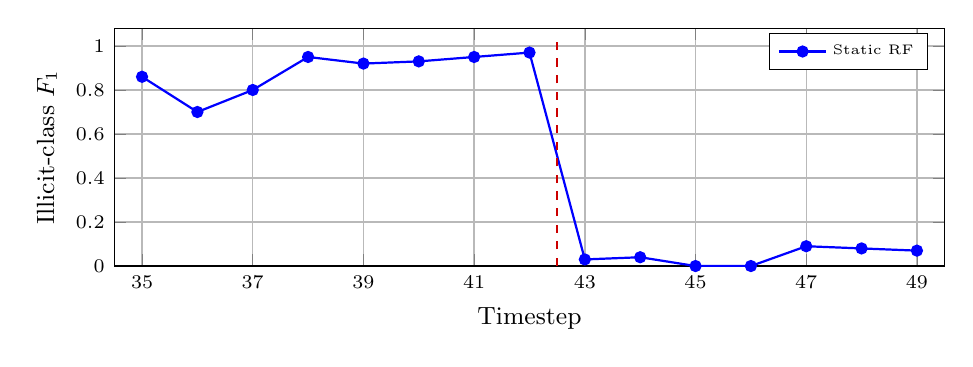
\begin{tikzpicture}
\begin{axis}[
  width=\linewidth, height=4.6cm,
  xlabel={Timestep}, ylabel={Illicit-class $F_1$},
  xmin=34.5, xmax=49.5, ymin=0, ymax=1.08,
  xtick={35,37,39,41,43,45,47,49},
  ytick={0,0.2,0.4,0.6,0.8,1.0},
  grid=both,
  grid style={line width=0.3pt, draw=gray!25},
  major grid style={line width=0.5pt, draw=gray!55},
  tick label style={font=\scriptsize},
  label style={font=\small},
  legend style={at={(0.98,0.98)}, anchor=north east, font=\tiny},
  mark size=1.8pt
]
\addplot[blue, mark=*, thick, mark options={fill=blue}] coordinates {
  (35,0.86)(36,0.70)(37,0.80)(38,0.95)
  (39,0.92)(40,0.93)(41,0.95)(42,0.97)
  (43,0.03)(44,0.04)(45,0.00)(46,0.00)
  (47,0.09)(48,0.08)(49,0.07)
};
\addlegendentry{Static RF}
\draw[red!80!black, dashed, thick]
  (axis cs:42.5,0) -- (axis cs:42.5,1.05)
  node[above, font=\tiny, text=red!80!black]{Drift $t{=}43$};
\end{axis}
\end{tikzpicture}
\caption{%
  Per-timestep illicit-class $F_1$ of the static Random Forest baseline.
  Performance is high and stable over steps 35--42 ($F_1 = 0.913$)
  then collapses sharply at step 43 ($F_1 = 0.032$).
}
\label{fig:drift}
\end{figure}

\subsubsection{Mitigation Results}

Table~\ref{tab:drift} compares the three retraining paradigms across
three seeds.
The \textbf{expanding window} recovers post-drift $F_1$ to
$0.164 \pm 0.055$ (single-seed peak $0.215$; precision $0.808$),
outperforming both static and sliding strategies.
The \textbf{sliding window} achieves only $F_1 = 0.087 \pm 0.017$:
the 10-step memory window captures timesteps 44--46, which contain as
few as 5 and 2 illicit transactions, causing severe label starvation.
Retaining all historical illicit representations (expanding window)
provides a richer, more stable decision boundary.

\begin{table}[t]
\centering
\caption{%
  Multi-seed drift mitigation results (mean $F_1 \pm$ std, seeds 0--2).
  Precision (P) and recall (R) for steps 43--49 are shown at seed~0.
}
\label{tab:drift}
\renewcommand{\arraystretch}{1.25}
\scriptsize
\begin{tabular}{@{}lccccc@{}}
\toprule
\textbf{Strategy}
  & $\boldsymbol{F_1^{35\text{-}42}}$
  & $\boldsymbol{F_1^{35\text{-}49}}$
  & $\boldsymbol{F_1^{43\text{-}49}}$
  & $\boldsymbol{P^{43\text{-}49}}$
  & $\boldsymbol{R^{43\text{-}49}}$ \\
\midrule
Static       & $0.913{\pm}0.000$ & $0.827{\pm}0.001$ & $0.032{\pm}0.000$ & 0.200 & 0.018 \\
Expanding    & $\mathbf{0.916{\pm}0.001}$ & $\mathbf{0.841{\pm}0.004}$ & $\mathbf{0.164{\pm}0.055}$ & \textbf{0.808} & \textbf{0.124} \\
Sliding (10) & $0.899{\pm}0.001$ & $0.819{\pm}0.001$ & $0.087{\pm}0.017$ & 0.533 & 0.047 \\
\bottomrule
\end{tabular}
\end{table}

% ════════════════════════════════════════════════════════════════════════════
\section{Discussion}
\label{sec:discussion}

\subsection{On Graph Feature Claims}

A common assertion in recent AML literature is that graph-topological
features are inherently necessary for high detection
performance~\cite{guo2023lb, lin2026wavelet, han2026featuregated}.
Our ablation directly contradicts this claim for \emph{static centrality
metrics applied to tree-ensemble classifiers}.
All four graph centrality features rank among the bottom 40\% by Gini
importance, and their addition to Random Forest yields a statistically
marginal gain of $+0.002$ in $F_1$.

We posit two explanations.
First, local transaction features already implicitly encode structural
information via the neighbourhood-aggregation features (columns 94--165)
provided by the Elliptic dataset~\cite{weber2019anti}, leaving minimal
residual signal for global centrality metrics.
Second, PageRank and degree centrality are global metrics computed over
the entire transaction history, conflating legitimate high-volume exchanges
with suspicious churning hubs in ways that the local features do not.

This does not preclude superior GNN approaches that exploit higher-order
structural motifs~\cite{bellei2024shape} or dynamic edge
formation~\cite{han2026featuregated}; it does require that researchers
rigorously ablate tabular baselines before claiming graph-topology
superiority.

\subsection{On Temporal Deployment Reliability}

A model that reports a strong aggregate test score ($F_1 = 0.827$)
predominantly due to early-window performance ($F_1 = 0.913$ at steps 35--42)
is functionally useless in the late window ($F_1 = 0.032$ at steps 43--49).
In live AML systems, detection capability must be sustained uniformly across
time; temporal decomposition of evaluation scores is therefore essential.

We provide three practical recommendations for operational AML pipelines:
\begin{itemize}
  \item \textbf{Use expanding-window retraining} rather than a fixed horizon
    to retain long-term historical illicit representations.
  \item \textbf{Monitor per-period label density.} Sudden drops in predicted
    illicit flagging may indicate behavioural drift rather than genuine
    cessation of illicit activity.
  \item \textbf{Avoid short sliding windows} during enforcement disruptions;
    label starvation across crackdown periods destroys model fidelity.
\end{itemize}

\subsection{Limitations}

{\v{S}}af{\'{a}}{\v{r}} et al.~\cite{safar2026enemy} raised concerns about
the opacity of the Elliptic feature labelling, which limits interpretability
of importance rankings.
Our work focuses on the publicly released feature set without attempting to
reverse-engineer anonymised feature semantics.
The 23-paper corpus also does not yet reach the target of 30--40 methods
papers set by our review protocol; expanding the literature search remains
future work.

% ════════════════════════════════════════════════════════════════════════════
\section{Conclusion}
\label{sec:conclusion}

This paper combined a structured taxonomy of 23 illicit Bitcoin detection
studies with a rigorous, seed-replicated empirical evaluation on the full
Elliptic benchmark.
Our experiments confirm that Random Forest achieves an illicit-class $F_1$
of $0.825 \pm 0.001$, faithfully reproducing the Weber et al.\ canonical
baseline.
A controlled ablation shows that four static graph centrality metrics add
only $+0.002$ to $F_1$ and rank outside the top 100 features by Gini
importance, challenging widespread claims of graph-feature superiority in
tabular AML tasks.
We further identify a catastrophic concept-drift collapse at timestep 43,
where static-model recall drops to $1.8\%$, and demonstrate that an
expanding-window retraining protocol recovers precision to $0.808$ and $F_1$
to $0.164 \pm 0.055$, while a 10-step sliding window suffers fatal label
starvation ($F_1 = 0.087 \pm 0.017$).

Future work will evaluate subgraph-level representations from the
Elliptic2 dataset~\cite{bellei2024shape}, active learning to accelerate
recovery after sudden regime shifts, and threshold-calibration strategies
to manage the precision-recall trade-off under dynamic retraining.

% ════════════════════════════════════════════════════════════════════════════
\section*{Acknowledgements}
The authors acknowledge the Elliptic research team for making the benchmark
dataset publicly available, and [Research Lab / Institution Name] for
computational resources.

% ════════════════════════════════════════════════════════════════════════════
\balance
\bibliographystyle{IEEEtran}
\bibliography{references}

\end{document}
